\chapter{Methodology}
\label{chap:four}

\section{\acl{ML}}

It is generally agreed upon that the term 
\ac{ML} refers to the field of study that gives computers the ability to learn 
without being explicitly programmed. This fact was first 
introduced by Arthur Samuel in 1959 \cite{Samuel1959}. However, note that the reference to this paper is used
loosely, as the term \ac{ML} was not directly used in the paper and it is rather 
a retrospective interpretation of the paper. 

The term \ac{ML} was more explicitly introduced by Tom M. Mitchell in 1997 \cite{Mitchell1997}:

\begin{defin}[Machine Learning]\label{de:ml}
    A computer program is said to learn from experience E with respect
    to some class of tasks T and performance measure P, if its performance at tasks in
    T, as measured by P, improves with experience E. 
\end{defin}

Typically, the experience E is represented by a dataset, which is used to train the model. 
We can generally say that \ac{ML} is the ability to get better at specified task by learning
from provided relevant data without problem domain specific programming of the computer.


Nowadays \ac{ML} is at the core of many applications that we use daily. The usecases range from
spam filters, recommendation systems, medical diagnosis, stock trading, and many more. Currently, 
machine learning is dominated by deep learning, which is a subfield of \ac{ML} that focuses on
deep neural networks that rely on large datasets in order to be able to generalize well.
On the other, hand traditional \ac{ML} algorithms are still widely used and are often the first choice
when the dataset is small or the problem is low dimensional. Whereas deep learning models
can be used in high frequency data, where the datasets are large enough to train the model, 
daily closing stock price prediction is a task that can be successfully solved with 
traditional \ac{ML} algorithms. As the datasets are much smaller. 


In general, cryptocurrencies
lie somewhere in the middle of the spectrum. Exactly as stocks, either high frequency or low frequency
data can be chosen based on the research question. The difference however is that cryptocurrencies 
are much more volatile than stocks, and they can have much higher dimensionality as we can use 
many technical analysis indicators to predict the price. 
That is why we will use a combination of
traditional \ac{ML} algorithms and deep learning models to predict the 
closing prices or returns of
various cryptocurrencies.

\ac{ML} algorithms can be divided into three main categories: supervised learning, unsupervised learning, and reinforcement learning.
As mentioned earlier, we will focus on supervised learning as the process of forecasting
can be easily transformed into a supervised learning problem where the input features
are historical or current data and the output is the future price or return.


It is important to note on the fundamental difference between machine learning and
traditional econometric models. In econometrics the focus is to uncover the underlying
relationship between the variables and to understand the size of contribution of each
feature. In machine learning, the focus is mainly on maximizing the performance metric for predictions and 
the magnitude of the effects usually remains unknown. This is definitely a weakness of machine learning
which researchers try to adress by developing new field of explainable \ac{AI}. 
Where they focus on developing models that are able to explain their predictions in a human understandable way.
They provide a significant promise for the use of \ac{ML} methods in finance in the future
where the interpretability of the model is crucial for customers or regulators in specific subfields.





\section{Ridge Linear Regression}

\section{Support Vector Machines}

\section{\acl{LSTM} \acl{RNN}s}

\section{\acl{PCA}}

\section{Time-Series Specifics}
Comment on stationarity in econoemtrics and ML.
\section{Proposed Forecasting Framework}

We propose a forecasting framework which is designed to compare the performance between using \ac{PCA} as a 
dimensionality reduction technique and using the raw data. 
The framework is shown in Figure \ref{fig:forecasting_framework}.
The preprocessing layer is responsible for cleaning the data, filling in missing values and tranforming 
the problem to supervised learning as described 
in \ref{chap:three}. Following stage is responsible for reducing the number of features. 
The first \ac{PCA} step transforms the data onto \textit{n} principal components and the filtering step
chooses the most important features such that their cumulative variance adds up to 95\%, 98\% or 99\%.
Following is the \ac{LSTM} reshaping layer that is responsible for transforming the data into a 3D tensor for 
the \ac{LSTM} \ac{RNN} as described 
in \ref{chap:three}. The most crucial layer is the forecasting layer that essentially consists of 3 parts.
Firstly, it normalizes the variables using robust scaler to ensure that the input features come from 
the same value range. Secondly, it uses grid search to search for the best
hyperparameters for the model. This is a cruical step as the change of dimensionality changes 
the optimal hyperparameters. Without this step it would be hard to establish any real
effects as the change in performance might be attributed to the change in suitability of hyperparameters.
Lastly, it trains the model and evaluates the performance using the best found model. This is the reason
why we abstract the metrics layer seperately to make it apparent that the metrics are calculated
on the best model found by the grid search. The metrics layer is also the layer where
we can statistically compare the significance of the difference between the models.
It is important to note that this framework is executed across all specified forecasting models, 
cryptocurrencies of interest, and forecasting horizons as we expect the effects
to be quite different for different models and forecasting horizons. 



\begin{figure}[!h]
    \centering
    \caption{Proposed Forecasting Framework}
        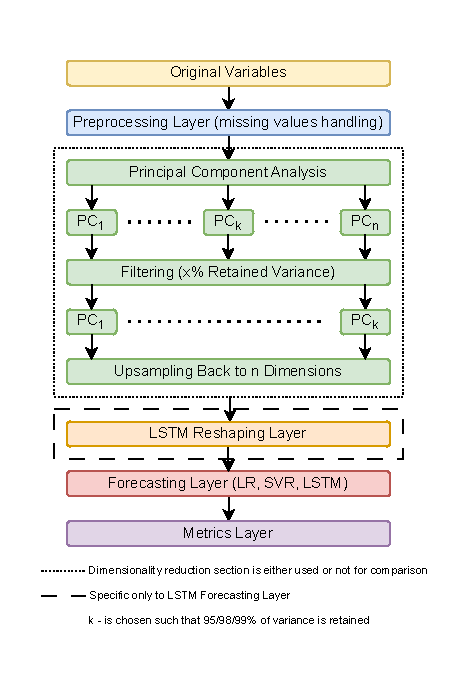
\includegraphics[width=1\textwidth]{Figures/Forecasting_framework.drawio.pdf}
    \label{fig:forecasting_framework}
\end{figure}